\documentclass[a4paper,12pt]{extarticle}
\usepackage[utf8x]{inputenc}
\usepackage[T1,T2A]{fontenc}
\usepackage[russian]{babel}
\usepackage{hyperref}
\usepackage{indentfirst}
\usepackage{listings}
\usepackage{color}
\usepackage{here}
\usepackage{array}
\usepackage{multirow}
\usepackage{graphicx}

\usepackage{caption}
\renewcommand{\lstlistingname}{Программа} % заголовок листингов кода

\bibliographystyle{ugost2008ls}

\usepackage{listings}
\lstset{ %
extendedchars=\true,
keepspaces=true,
language=C,						% choose the language of the code
basicstyle=\footnotesize,		% the size of the fonts that are used for the code
numbers=left,					% where to put the line-numbers
numberstyle=\footnotesize,		% the size of the fonts that are used for the line-numbers
stepnumber=1,					% the step between two line-numbers. If it is 1 each line will be numbered
numbersep=5pt,					% how far the line-numbers are from the code
backgroundcolor=\color{white},	% choose the background color. You must add \usepackage{color}
showspaces=false				% show spaces adding particular underscores
showstringspaces=false,			% underline spaces within strings
showtabs=false,					% show tabs within strings adding particular underscores
frame=single,           		% adds a frame around the code
tabsize=2,						% sets default tabsize to 2 spaces
captionpos=t,					% sets the caption-position to top
breaklines=true,				% sets automatic line breaking
breakatwhitespace=false,		% sets if automatic breaks should only happen at whitespace
escapeinside={\%*}{*)},			% if you want to add a comment within your code
postbreak=\raisebox{0ex}[0ex][0ex]{\ensuremath{\color{red}\hookrightarrow\space}},
texcl=true,
inputpath=listings,                     % директория с листингами
}

\usepackage[left=2cm,right=2cm,
top=2cm,bottom=2cm,bindingoffset=0cm]{geometry}

%% Нумерация картинок по секциям
\usepackage{chngcntr}
\counterwithin{figure}{section}
\counterwithin{table}{section}

%%Точки нумерации заголовков
\usepackage{titlesec}
\titlelabel{\thetitle.\quad}
\usepackage[dotinlabels]{titletoc}

%% Оформления подписи рисунка
\addto\captionsrussian{\renewcommand{\figurename}{Рисунок}}
\captionsetup[figure]{labelsep = period}

%% Подпись таблицы
\DeclareCaptionFormat{hfillstart}{\hfill#1#2#3\par}
\captionsetup[table]{format=hfillstart,labelsep=newline,justification=centering,skip=-10pt,textfont=bf}

%% Путь к каталогу с рисунками
\graphicspath{{fig/}}


\begin{document}	% начало документа

% Титульная страница
\begin{titlepage}	% начало титульной страницы

	\begin{center}		% выравнивание по центру

		\large Санкт-Петербургский политехнический университет Петра Великого\\
		\large Институт компьютерных наук и технологий \\
		\large Кафедра компьютерных систем и программных технологий\\[6cm]
		% название института, затем отступ 6см
		
		\huge Телекоммуникационные технологии\\[0.5cm] % название работы, затем отступ 0,5см
		\large Отчет по лабораторной работе №6\\[0.1cm]
		\large Цифровая модуляция\\[5cm]

	\end{center}


	\begin{flushright} % выравнивание по правому краю
		\begin{minipage}{0.25\textwidth} % врезка в половину ширины текста
			\begin{flushleft} % выровнять её содержимое по левому краю

				\large\textbf{Работу выполнил:}\\
				\large Графов Д.И.\\
				\large {Группа:} 33531/2\\
				
				\large \textbf{Преподаватель:}\\
				\large Богач Н.В.

			\end{flushleft}
		\end{minipage}
	\end{flushright}
	
	\vfill % заполнить всё доступное ниже пространство

	\begin{center}
	\large Санкт-Петербург\\
	\large \the\year % вывести дату
	\end{center} % закончить выравнивание по центру

\thispagestyle{empty} % не нумеровать страницу
\end{titlepage} % конец титульной страницы

\vfill % заполнить всё доступное ниже пространство


% Содержание
% Содержание
\renewcommand\contentsname{\centerline{Содержание}}
\tableofcontents
\newpage




\section{Цель работы}
Изучение амплитудной модуляции/демодуляции сигнала.

\section{Программа работы}
Сгенерировать однотональный сигнал низкой частоты.

Выполнить амплитудную модуляцию (АМ) сигнала по закону u(t) = (1 + MUm cos Ωt) cos(ω0t + φ0). 

Получить спектр модулированного сигнала.

Выполнить модуляцию с подавлением несущей
u(t) = MUm cos(Ωt) cos(ω0t + φ0). Получить спектр.

Выполнить однополосную модуляцию:
U m 􏰀N
u(t) = Um cos(Ωt) cos(ω0t+φ0)+ 2 положив n=1

Выполнить синхронное детектирование и получить исходный однополосный сигнал.

Рассчитать КПД модуляции.\\


\section{Теоретическая информация}
Амплитудная модуляция — вид модуляции, при которой изменяемым параметром несущего сигнала является его амплитуда. \\ Пусть
S(t) — информационный сигнал, |S(t)|<1,
Uc(t) — несущее колебание.
Тогда \\амплитудно-модулированный сигнал Uam(t) может быть записан следующим образом:\\
Uam(t)=Uc(t)*[1+m*S(t)].\\
Здесь m — некоторая константа, называемая коэффициентом модуляции. Формула описывает несущий сигнал Uc(t), модулированный по амплитуде сигналом S(t) с коэффициентом модуляции m. Предполагается также, что выполнены условия:
|S(t)|<1, 0<m<=1.

Выполнение условий необходимо для того, чтобы выражение в квадратных скобках в всегда было положительным. Если оно может принимать отрицательные значения в какой-то момент времени, то происходит так называемая перемодуляция (избыточная модуляция). Простые демодуляторы (типа квадратичного детектора) демодулируют такой сигнал с сильными искажениями. 

Демодуляция — процесс, обратный модуляции колебаний, выделение информационного (модулирующего) сигнала из модулированного колебания высокой (несущей) частоты. 

 Одним из самых распространенных методов демодуляции амплитудно-модулированных сигналов является синхронное детектирование. При синхронном детектировании амплитудно-модулированный сигнал умножается на опорное немодулированное колебание с частотой несущего колебания, затем получившийся сигнал пропускается через фильтр нижних частот. В результате умножения получается сигнал, состоящий из двух слагаемых, первое из которых прямо пропорционально исходному модулирующему сигналу, а второе — амплитудно-модулированному сигналу с удвоенной несущей частотой. Второе слагаемое подавляет фильтр нижних частот, таким образом оставляется сигнал, прямо пропорциональный исходному информационному сигналу.





\section{Ход выполнения работы}

\subsection{Листинг}

\lstinputlisting[
	label=code:lab12
	caption={lab4.py},% для печати символ '_' требует выходной символ '\'
]{lab4.py}
\parindent=1cm % командна \lstinputlisting сбивает параментры отступа

\subsection{Граффики}

\begin{figure}[H]
	\begin{center}
		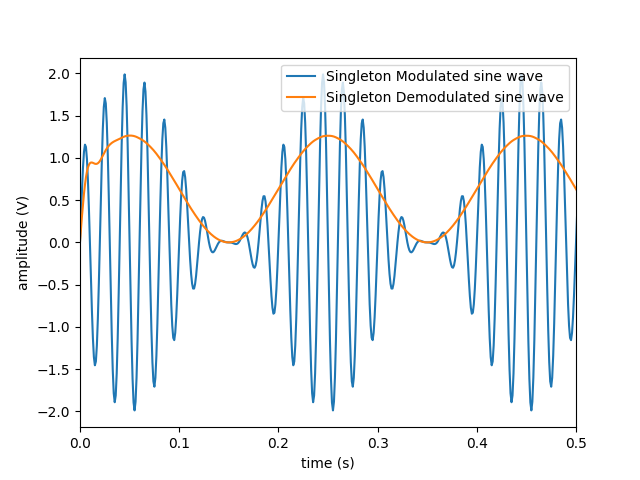
\includegraphics[scale=0.7]{1}
		\caption{амплитудная модуляция и демодуляция} 
		\label{pic:1} % название для ссылок внутри кода
	\end{center}
\end{figure}

\begin{figure}[H]
	\begin{center}
		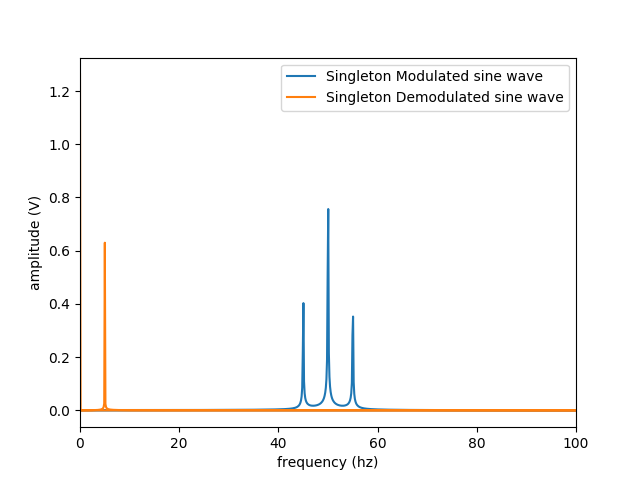
\includegraphics[scale=0.7]{2}
		\caption{спектр промодулированного сигнала} 
		\label{pic:triangle_spectrum} % название для ссылок внутри кода
	\end{center}
\end{figure}

\begin{figure}[H]
	\begin{center}
		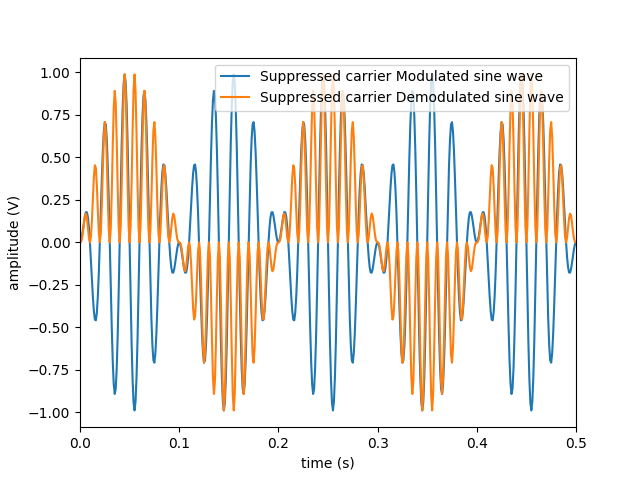
\includegraphics[scale=0.7]{3}
		\caption{модуляция и демодуляция с подавлением несущей} 
		\label{pic:triangle_spectrum} % название для ссылок внутри кода
	\end{center}
\end{figure}

\begin{figure}[H]
	\begin{center}
		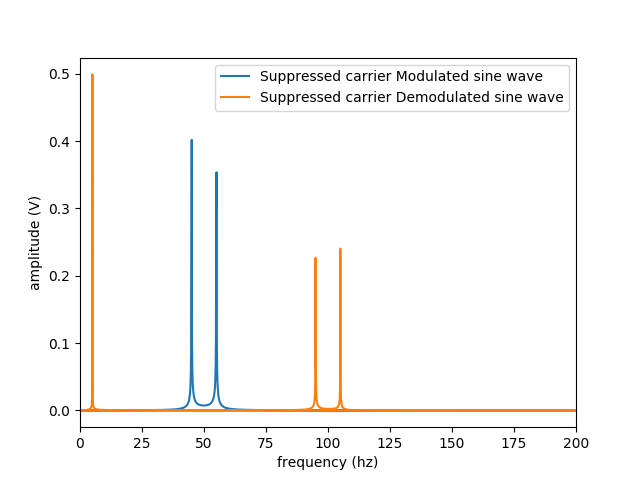
\includegraphics[scale=0.7]{4}
		\caption{спектр промодулированного сигнала} 
		\label{pic:triangle_spectrum} % название для ссылок внутри кода
	\end{center}
\end{figure}

\begin{figure}[H]
	\begin{center}
		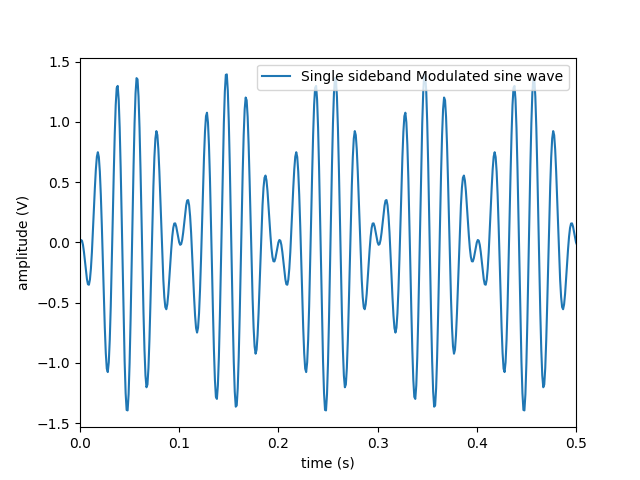
\includegraphics[scale=0.7]{5}
		\caption{однополосная модуляция} 
		\label{pic:triangle_spectrum} % название для ссылок внутри кода
	\end{center}
\end{figure}

\begin{figure}[H]
	\begin{center}
		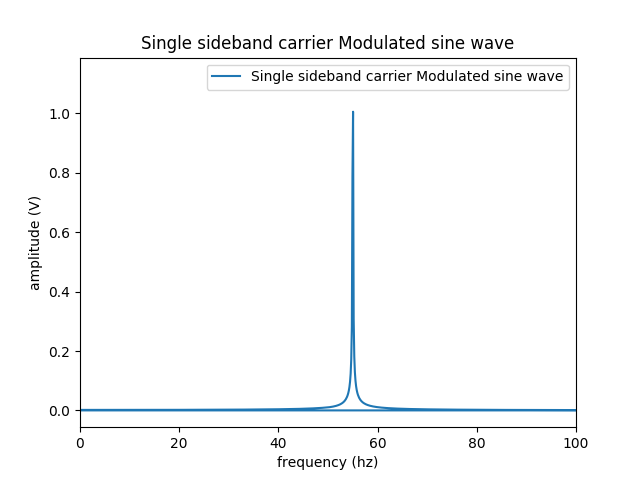
\includegraphics[scale=0.7]{6}
		\caption{спектр промодулированного сигнала} 
		\label{pic:triangle_spectrum} % название для ссылок внутри кода
	\end{center}
\end{figure}

\section{Выводы}
В данной работе были рассмотренны амплитудная модуляция и демодуляция, модуляция с подавлением нусещей и однополосная модуляция, а так же их спектры. 
\end{document}
